\documentclass[11pt,preprint]{elsarticle}

\usepackage{lmodern}
%%%% My spacing
\usepackage{setspace}
\setstretch{1.2}
\DeclareMathSizes{12}{14}{10}{10}

% Wrap around which gives all figures included the [H] command, or places it "here". This can be tedious to code in Rmarkdown.
\usepackage{float}
% The [H] wrapper for figures is switched off, so that figures float to the top or bottom of a page as set by fig.pos in the Rmd and pages are not left half empty
% \let\origfigure\figure
% \let\endorigfigure\endfigure
% \renewenvironment{figure}[1][2] {
%     \expandafter\origfigure\expandafter[H]
% } {
%     \endorigfigure
% }

\let\origtable\table
\let\endorigtable\endtable
\renewenvironment{table}[1][2] {
    \expandafter\origtable\expandafter[H]
} {
    \endorigtable
}


\usepackage{ifxetex,ifluatex}
\usepackage{fixltx2e} % provides \textsubscript
\ifnum 0\ifxetex 1\fi\ifluatex 1\fi=0 % if pdftex
  \usepackage[T1]{fontenc}
  \usepackage[utf8]{inputenc}
\else % if luatex or xelatex
  \ifxetex
    \usepackage{mathspec}
    \usepackage{xltxtra,xunicode}
  \else
    \usepackage{fontspec}
  \fi
  \defaultfontfeatures{Mapping=tex-text,Scale=MatchLowercase}
  \newcommand{\euro}{€}
\fi

\usepackage{amssymb, amsmath, amsthm, amsfonts}

\def\bibsection{\section*{References}} %%% Make "References" appear before bibliography


\usepackage[numbers]{natbib}

\usepackage{longtable}
\usepackage[margin=2.3cm,bottom=2cm,top=2.5cm, includefoot]{geometry}
\usepackage{fancyhdr}
\usepackage[bottom, hang, flushmargin]{footmisc}
\usepackage{graphicx}
\numberwithin{equation}{section}
\numberwithin{figure}{section}
\numberwithin{table}{section}
\setlength{\parindent}{0cm}
\setlength{\parskip}{1.3ex plus 0.5ex minus 0.3ex}
\usepackage{textcomp}
\renewcommand{\headrulewidth}{0.2pt}
\renewcommand{\footrulewidth}{0.3pt}

\usepackage{array}
\newcolumntype{x}[1]{>{\centering\arraybackslash\hspace{0pt}}p{#1}}

%%%%  Remove the "preprint submitted to" part. Don't worry about this either, it just looks better without it:
\makeatletter
\def\ps@pprintTitle{%
  \let\@oddhead\@empty
  \let\@evenhead\@empty
  \let\@oddfoot\@empty
  \let\@evenfoot\@oddfoot
}
\makeatother

 \def\tightlist{} % This allows for subbullets!

\usepackage{hyperref}
\hypersetup{breaklinks=true,
            bookmarks=true,
            colorlinks=true,
            citecolor=blue,
            urlcolor=blue,
            linkcolor=blue,
            pdfborder={0 0 0}}


% The following packages allow huxtable to work:
\usepackage{siunitx}
\usepackage{multirow}
\usepackage{hhline}
\usepackage{calc}
\usepackage{tabularx}
\usepackage{booktabs}
\usepackage{caption}


\newenvironment{columns}[1][]{}{}

\newenvironment{column}[1]{\begin{minipage}{#1}\ignorespaces}{%
\end{minipage}
\ifhmode\unskip\fi
\aftergroup\useignorespacesandallpars}

\def\useignorespacesandallpars#1\ignorespaces\fi{%
#1\fi\ignorespacesandallpars}

\makeatletter
\def\ignorespacesandallpars{%
  \@ifnextchar\par
    {\expandafter\ignorespacesandallpars\@gobble}%
    {}%
}
\makeatother


% definitions for citeproc citations
\NewDocumentCommand\citeproctext{}{}
\NewDocumentCommand\citeproc{mm}{%
\href{\#cite.\detokenize{#1}}{#2}\nocite{#1}}

\makeatletter
% allow citations to break across lines
\let\@cite@ofmt\@firstofone
% avoid brackets around text for \cite:
\def\@biblabel#1{}
\def\@cite#1#2{{#1\if@tempswa , #2\fi}}
\makeatother
\newlength{\cslhangindent}
\setlength{\cslhangindent}{1.5em}
\newlength{\csllabelwidth}
\setlength{\csllabelwidth}{3em}
\newenvironment{CSLReferences}[2] % #1 hanging-indent, #2 entry-spacing
{\begin{list}{}{%
	\setlength{\itemindent}{0pt}
	\setlength{\leftmargin}{0pt}
	\setlength{\parsep}{0pt}
	% turn on hanging indent if param 1 is 1
	\ifodd #1
	\setlength{\leftmargin}{\cslhangindent}
	\setlength{\itemindent}{-1\cslhangindent}
	\fi
	% set entry spacing
	\setlength{\itemsep}{#2\baselineskip}}}
{\end{list}}

\usepackage{calc}
\newcommand{\CSLBlock}[1]{\hfill\break\parbox[t]{\linewidth}{\strut\ignorespaces#1\strut}}
\newcommand{\CSLLeftMargin}[1]{\parbox[t]{\csllabelwidth}{\strut#1\strut}}
\newcommand{\CSLRightInline}[1]{\parbox[t]{\linewidth - \csllabelwidth}{\strut#1\strut}}
\newcommand{\CSLIndent}[1]{\hspace{\cslhangindent}#1}


\urlstyle{same}  % don't use monospace font for urls
\setlength{\parindent}{0pt}
\setlength{\parskip}{6pt plus 2pt minus 1pt}
\setlength{\emergencystretch}{3em}  % prevent overfull lines
\setcounter{secnumdepth}{5}

%%% Use protect on footnotes to avoid problems with footnotes in titles
\let\rmarkdownfootnote\footnote%
\def\footnote{\protect\rmarkdownfootnote}
\IfFileExists{upquote.sty}{\usepackage{upquote}}{}

%%% Include extra packages specified by user
\renewcommand{\topfraction}{0.9}
\renewcommand{\bottomfraction}{0.8}
\renewcommand{\textfraction}{0.07}
\renewcommand{\floatpagefraction}{0.8}
\setcounter{topnumber}{2}
\setcounter{bottomnumber}{2}
\setcounter{totalnumber}{3}
\usepackage{placeins}

%%% Hard setting column skips for reports - this ensures greater consistency and control over the length settings in the document.
%% page layout
%% paragraphs
\setlength{\baselineskip}{12pt plus 0pt minus 0pt}
\setlength{\parskip}{12pt plus 0pt minus 0pt}
\setlength{\parindent}{0pt plus 0pt minus 0pt}
%% floats
\setlength{\floatsep}{12pt plus 0 pt minus 0pt}
\setlength{\textfloatsep}{20pt plus 0pt minus 0pt}
\setlength{\intextsep}{14pt plus 0pt minus 0pt}
\setlength{\dbltextfloatsep}{20pt plus 0pt minus 0pt}
\setlength{\dblfloatsep}{14pt plus 0pt minus 0pt}
%% maths
\setlength{\abovedisplayskip}{12pt plus 0pt minus 0pt}
\setlength{\belowdisplayskip}{12pt plus 0pt minus 0pt}
%% lists
\setlength{\topsep}{10pt plus 0pt minus 0pt}
\setlength{\partopsep}{3pt plus 0pt minus 0pt}
\setlength{\itemsep}{5pt plus 0pt minus 0pt}
\setlength{\labelsep}{8mm plus 0mm minus 0mm}
\setlength{\parsep}{\the\parskip}
\setlength{\listparindent}{\the\parindent}
%% verbatim
\setlength{\fboxsep}{5pt plus 0pt minus 0pt}



\begin{document}



\begin{frontmatter}  %

\title{A Global Balanced Index Fund Under a Constrained Mandate}

% Set to FALSE if wanting to remove title (for submission)




\author[Add1]{Diaz Sangeve}
\ead{24991422@sun.ac.za}





\address[Add1]{Stellenbosch University, Stellenbosch, South Africa}

\cortext[cor]{Corresponding author: Diaz Sangeve}

\begin{abstract}
\small{
This report constructs a Global Balanced Index Fund from traded global
and local indexes under a mandate that limits bonds to 25 percent,
equities to 75 percent, commodities to 15 percent, any single asset to
35 percent and offshore exposure to 60 percent, with quarterly
rebalancing, a ten year estimation look-back and a five year minimum
history. Ten year bond indexes are first built from yields. Four
portfolio rules that all satisfy the mandate on every rebalance date are
compared from 2020 to 2026, namely constrained equal weight, minimum
variance, constrained risk parity and maximum Sharpe. The bond and
global limits bind for almost every rule and shape the portfolios more
than the choice of rule. Maximum Sharpe earned the highest return
through a concentrated position in United States equity, while
constrained risk parity offered the most balanced combination of return,
diversification and low turnover without relying on expected returns,
and held up best in the stressed years of 2020 to 2022. Constrained risk
parity is recommended.
}
\end{abstract}

\vspace{1cm}


\begin{keyword}
\footnotesize{
Portfolio construction \sep Risk parity \sep Minimum variance
\sep Efficient frontier \sep Constraints \\
\vspace{0.3cm}
}
\footnotesize{
\textit{JEL classification} G11 \sep G15 \sep C61
}
\end{keyword}



\vspace{0.5cm}

\end{frontmatter}

\setcounter{footnote}{0}



%________________________
% Header and Footers
%%%%%%%%%%%%%%%%%%%%%%%%%%%%%%%%%
\pagestyle{fancy}
\chead{}
\rhead{}
\lfoot{}
\rfoot{\footnotesize Page \thepage}
\lhead{}
%\rfoot{\footnotesize Page \thepage } % "e.g. Page 2"
\cfoot{}

%\setlength\headheight{30pt}
%%%%%%%%%%%%%%%%%%%%%%%%%%%%%%%%%
%________________________

\headsep 35pt % So that header does not go over title




\section{\texorpdfstring{Introduction
\label{Intro}}{Introduction }}\label{introduction}

A balanced index fund must combine asset classes so that no single
market drives its outcome, while respecting the limits its mandate sets.
This report builds such a fund from traded global and local indexes and
compares four rules for setting its weights. Section \ref{Data} sets out
the mandate and the approach, Section \ref{Universe} describes the
universe, the construction of bond indexes from yields and the
correlation structure, Section \ref{Method} defines the portfolio rules,
Section \ref{Results} compares the portfolios within the mandate,
Section \ref{Backtest} evaluates them out of sample and Section
\ref{Recommend} gives the scorecard, the recommendation and robustness
checks. Section \ref{Conclusion} concludes.

\section{\texorpdfstring{Mandate, Data and Approach
\label{Data}}{Mandate, Data and Approach }}\label{mandate-data-and-approach}

\subsection{The Mandate and the Order of the
Analysis}\label{the-mandate-and-the-order-of-the-analysis}

This question builds a Global Balanced Index Fund from traded indexes
under a mandate with nine conditions. The fund must be long only, use a
look-back of at least ten years for any mean or covariance estimate,
hold no asset with less than five years of returns, rebalance quarterly,
and keep bonds and credit at or below 25 percent, equities at or below
75 percent, commodities at or below 15 percent, any single asset at or
below 35 percent and offshore exposure at or below 60 percent. The
analysis uses monthly returns and estimates the covariance matrix from
data after 2010, as the brief instructs.

The question invites several angles, so the analysis is built as a
sequence. It first defines the universe and checks which assets the five
year rule allows, then builds the bond indexes that the brief asks for
from yields, and studies how the assets move together. It then
constructs four portfolios that all satisfy every condition of the
mandate, namely a constrained equal weight baseline, minimum variance,
constrained risk parity and maximum Sharpe ratio, and compares them
through the efficient frontier, the split between capital and risk, how
hard each leans on the mandate, and an out-of-sample backtest from 2020.
It closes with a recommendation and robustness checks.

Two data points shape the design. The brief mentions description files
that are not in the data folder, so the universe is built from the files
named in the brief's code. There is also no exchange rate in the data,
so offshore assets are measured in dollars and local assets in rand. The
backtest therefore reflects a fund whose offshore holdings are currency
hedged, ignoring the cost of hedging, which is stated wherever it
matters.

\section{\texorpdfstring{The Universe and Its Inputs
\label{Universe}}{The Universe and Its Inputs }}\label{the-universe-and-its-inputs}

\subsection{The Investable Universe}\label{the-investable-universe}

The universe combines four offshore regional equity indexes and United
States real estate, three ten year government bond indexes built from
yields, a broad commodity index and gold, the local large and mid cap
indexes with two local factor indexes, and the local bond, inflation
linked bond and listed property indexes. Regional equity indexes are
preferred to the all country index, since holding both would double
count the same shares. Listed property counts towards the equity limit,
since it trades as equity, and inflation linked bonds count towards the
bond limit. Of the three local factor indexes, low volatility only
starts in 2024, so the five year rule rules it out and momentum and
value are chosen.

\begin{figure}[H]

{\centering 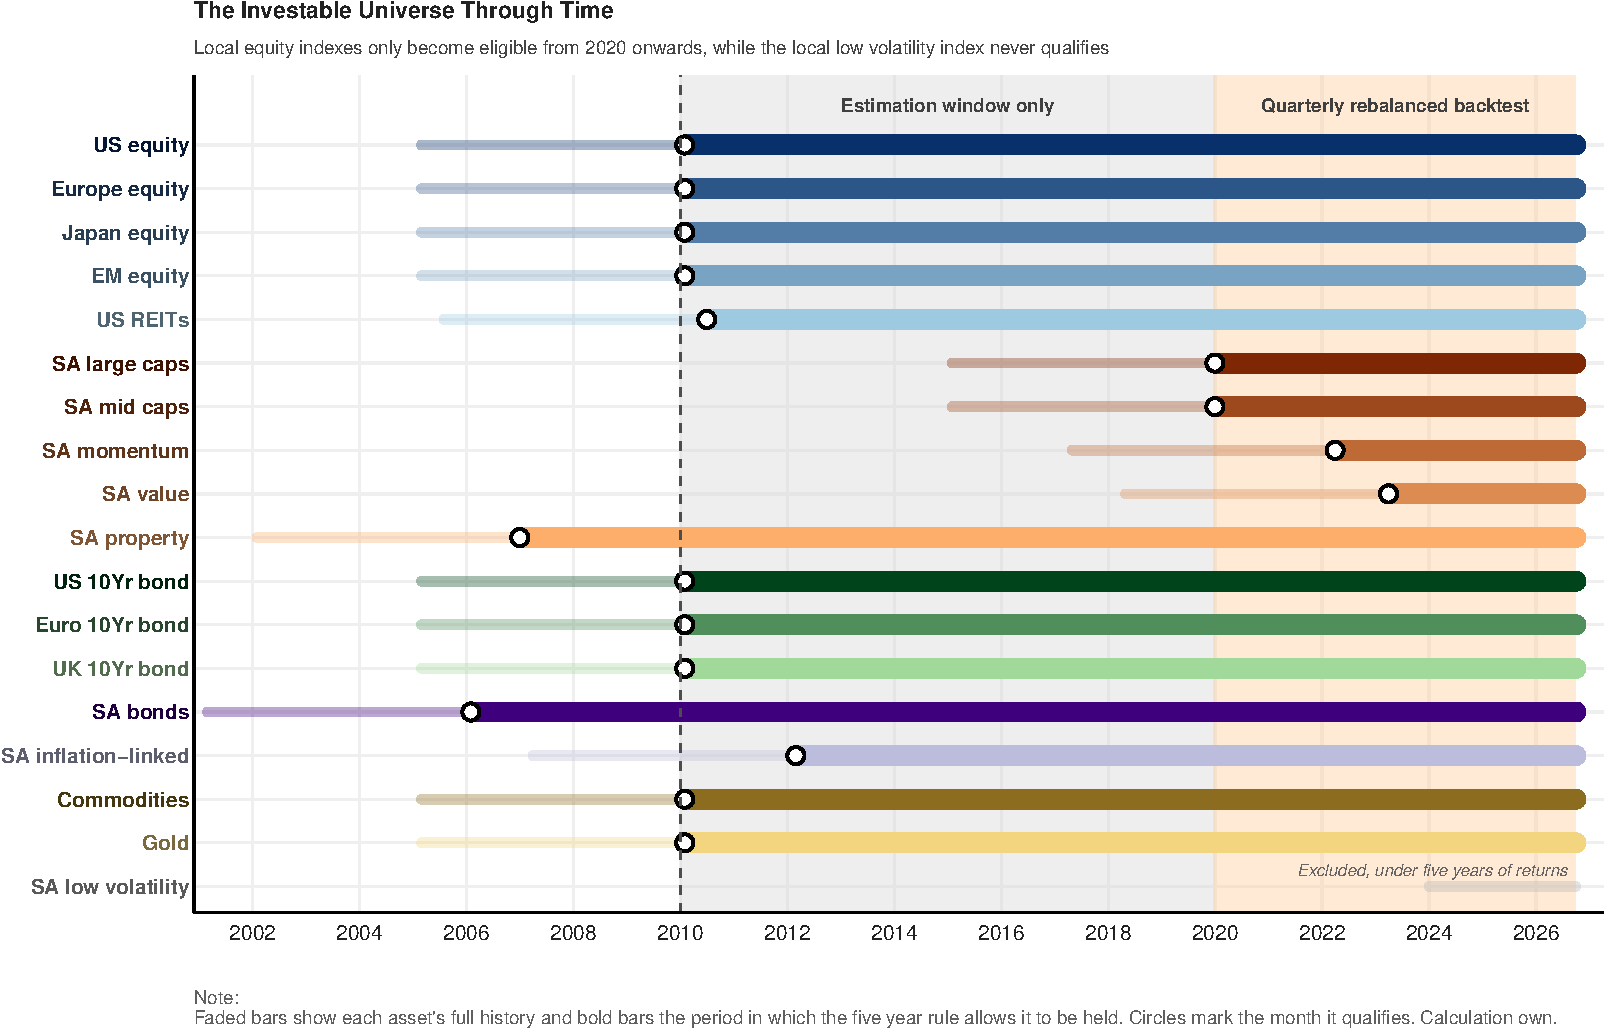
\includegraphics[width=1\linewidth]{Question4_files/figure-latex/q4_universe-1} 

}

\caption{The Investable Universe Through Time}\label{fig:q4_universe}
\end{figure}

The timeline shows why the backtest starts at the end of 2019. A
look-back of at least ten years on data after 2010 first exists in
December 2019, and the local large and mid cap indexes, whose returns
begin in January 2015, qualify on that same date. Local momentum
qualifies in March 2022 and local value in March 2023, so the universe
grows from 15 to 17 assets over the backtest. For assets with less than
ten years of history, the estimation window is still the full window
from 2010, and each pair's correlation is estimated over the months both
assets have returns.

\subsection{Building Bond Indexes From
Yields}\label{building-bond-indexes-from-yields}

The brief provides ten year government bond yields, not returns, so a
total return index must be built first. Each month the index is assumed
to buy a ten year par bond, whose coupon equals that month's yield. A
month later the bond has nine years and eleven months left and is
repriced at the new yield, and its return is the price change plus a
month of coupon income. This captures both the income from a bond and
the capital loss when yields rise, and the full repricing also captures
convexity, which a duration approximation would miss when yields move
sharply.

\begin{figure}[H]

{\centering 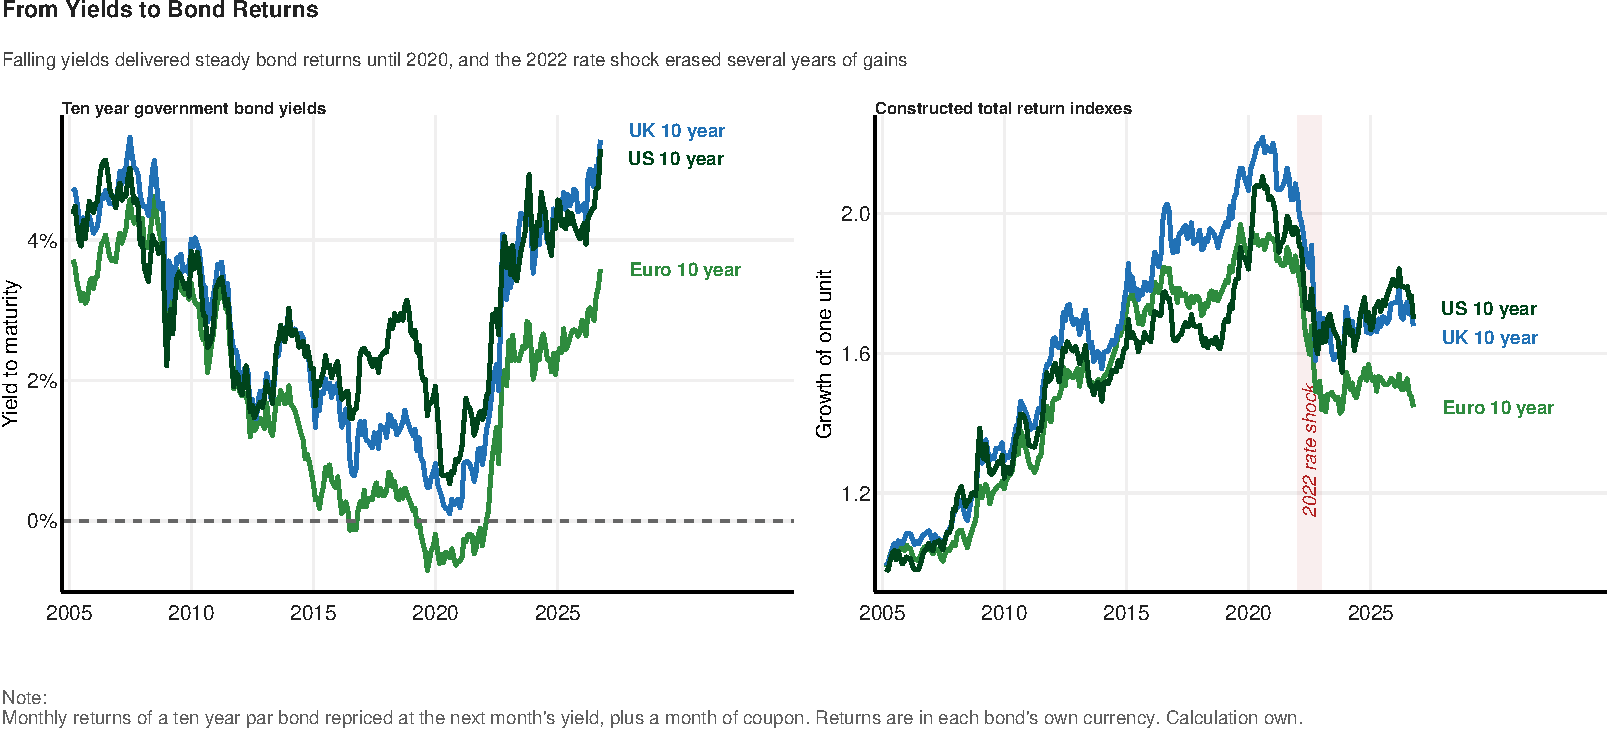
\includegraphics[width=1\linewidth]{Question4_files/figure-latex/q4_bonds-1} 

}

\caption{From Yields to Bond Returns}\label{fig:q4_bonds}
\end{figure}

The constructed indexes behave as expected. The United States index
returned 2.5 percent a year since 2005 with volatility of 7.5 percent,
and the euro index, whose yield was below zero in 37 months, returned
only 1.7 percent. In 2022 the three indexes lost between 16.4 percent
and 22.1 percent as central banks raised rates, which shows that
government bonds can fall together with equities when inflation is the
shock.

\subsection{How the Assets Move
Together}\label{how-the-assets-move-together}

Diversification depends on correlation, so the chord diagram links every
pair of assets whose monthly returns since 2010 have a correlation above
0.5, with wider and deeper blue chords for stronger links, and draws red
chords for pairs with a correlation below -0.15.

\begin{figure}[H]

{\centering 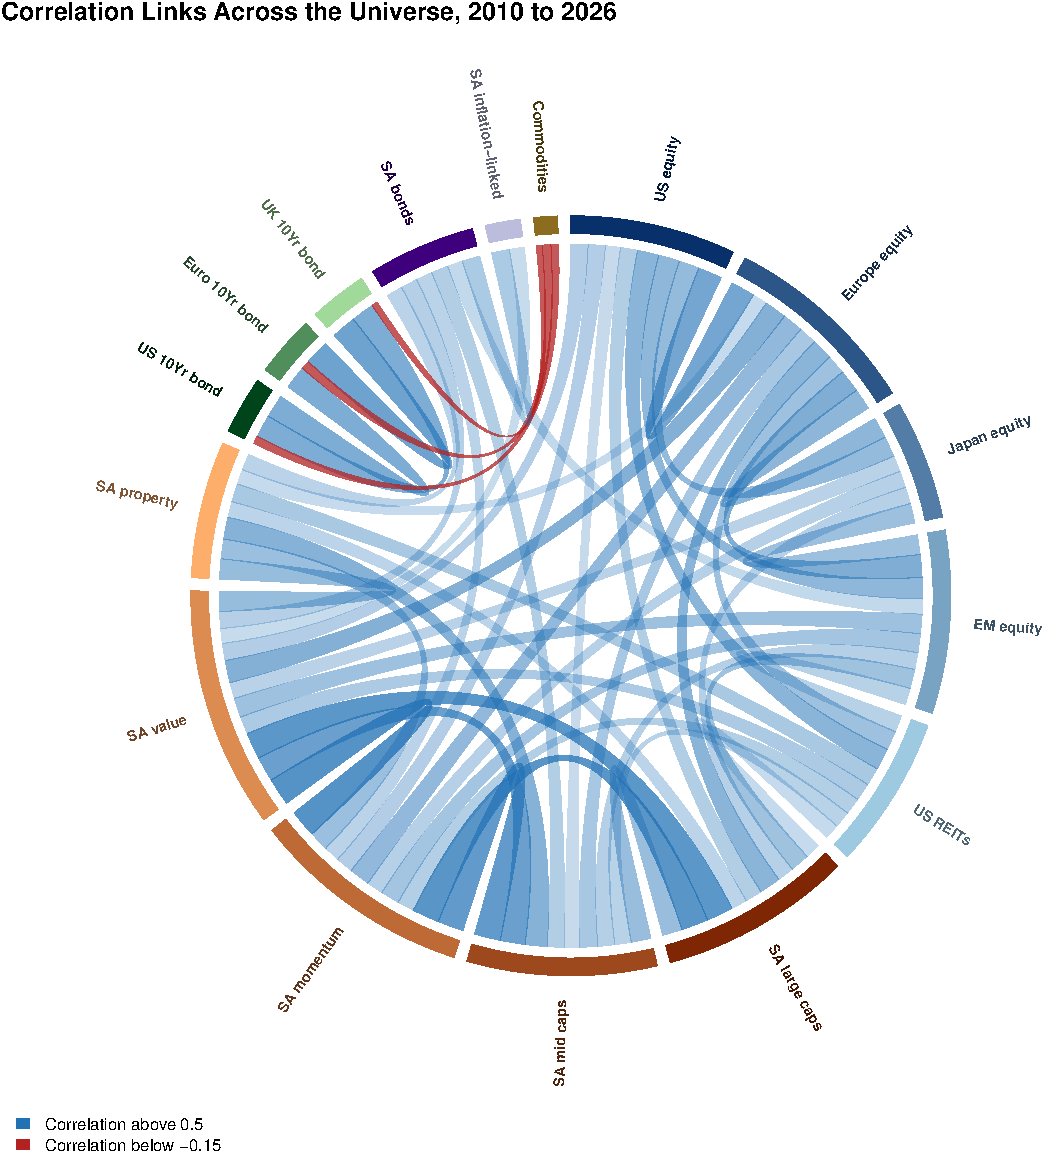
\includegraphics[width=1\linewidth]{Question4_files/figure-latex/q4_chord-1} 

}

\caption{Correlation Links Across the Universe, 2010 to 2026}\label{fig:q4_chord}
\end{figure}

The diagram is dominated by two dense clusters. Local equity indexes are
tightly linked to one another, with an average correlation of 0.86, and
offshore equities form a second cluster, while the average correlation
between the two clusters is lower, at 0.61, partly because local returns
are in rand and offshore returns in dollars, and the rand tends to
weaken when global markets fall. Bonds connect mainly to each other, and
the only red chords link the three offshore bonds with commodities,
which tend to rise when inflation pushes bond yields up. Gold does not
appear at all, since its strongest correlation with any asset is only
0.47, which makes it the most independent asset in the universe and
explains why every optimiser holds it.

\section{\texorpdfstring{Portfolio Rules
\label{Method}}{Portfolio Rules }}\label{portfolio-rules}

\subsection{Four Ways to Build the
Portfolio}\label{four-ways-to-build-the-portfolio}

All four portfolios share the same inputs and the same constraints, so
their differences come only from the rule that sets the weights. At each
quarter end the covariance matrix and expected returns are estimated
from monthly returns since January 2010. Correlations are shrunk a
quarter of the way towards their average and expected returns half way
towards their grand mean, since sample means are the noisiest input to
any optimiser, and the matrix is then made positive definite. The
constraints enter the optimisers as linear restrictions, with the five
year rule applied by dropping assets that have fewer than 60 monthly
returns on the rebalance date.

The constrained equal weight portfolio is the closest portfolio to equal
weights that satisfies the mandate and uses no estimates, so it is the
naive benchmark. Minimum variance uses only the covariance matrix.
Constrained risk parity searches for the weights whose contributions to
portfolio risk are as close to equal as the mandate allows, using
numerical optimisation. Maximum Sharpe maximises expected return per
unit of volatility and is the only rule that relies on expected returns,
solved as a quadratic programme by rescaling the weights and rewriting
every cap relative to the scale.

Across 27 rebalance dates and four rules, the largest breach of any
limit is 0.000000, so every portfolio satisfies the mandate on every
date.

\section{\texorpdfstring{The Portfolios Within the Mandate
\label{Results}}{The Portfolios Within the Mandate }}\label{the-portfolios-within-the-mandate}

\subsection{The Efficient Frontier and the Cost of the
Mandate}\label{the-efficient-frontier-and-the-cost-of-the-mandate}

The frontier view shows what the mandate costs. On the latest rebalance
date, the solid line is the efficient frontier within the mandate and
the dashed line is the frontier with only the long-only condition. Each
asset is marked by its family colour, and the four rules are marked as
diamonds.

\begin{figure}[H]

{\centering 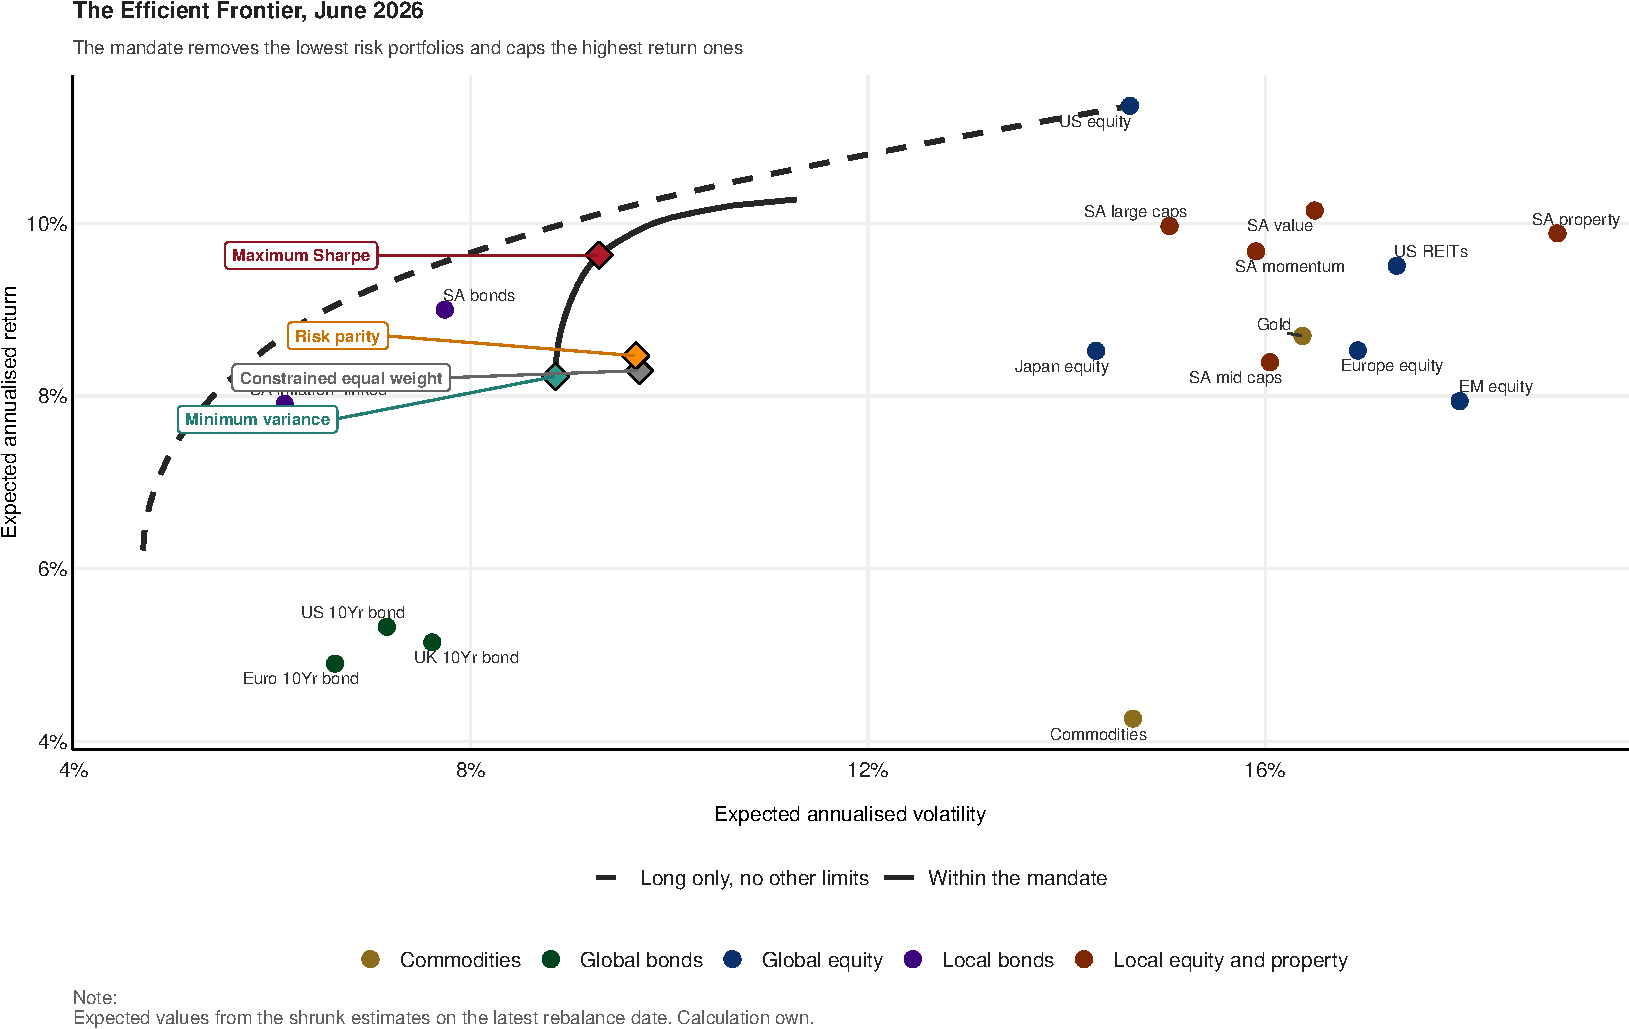
\includegraphics[width=1\linewidth]{Question4_files/figure-latex/q4_frontier-1} 

}

\caption{The Efficient Frontier, June 2026}\label{fig:q4_frontier}
\end{figure}

The mandate binds most at the low risk end. With only the long-only
condition, the least volatile portfolio has an expected volatility of
4.7 percent, built mostly from bonds and led by local inflation linked
bonds, but the 25 percent bond limit and the 60 percent global limit
push the least volatile mandate portfolio up to 8.9 percent. The 35
percent single asset cap also stops the frontier from reaching the high
return end, where United States equity sits on its own. Within the
mandate, minimum variance sits at the lowest point of the frontier and
maximum Sharpe on its upper section, while risk parity and the equal
weight baseline sit just inside it, since neither uses expected returns.

\subsection{Weights Along the
Frontier}\label{weights-along-the-frontier}

The frontier figure shows the risk and return that the mandate allows,
but not which assets deliver them. The weights of every portfolio on the
mandate frontier on the latest rebalance date are stacked against its
volatility, with the four rules marked.

\begin{figure}[H]

{\centering 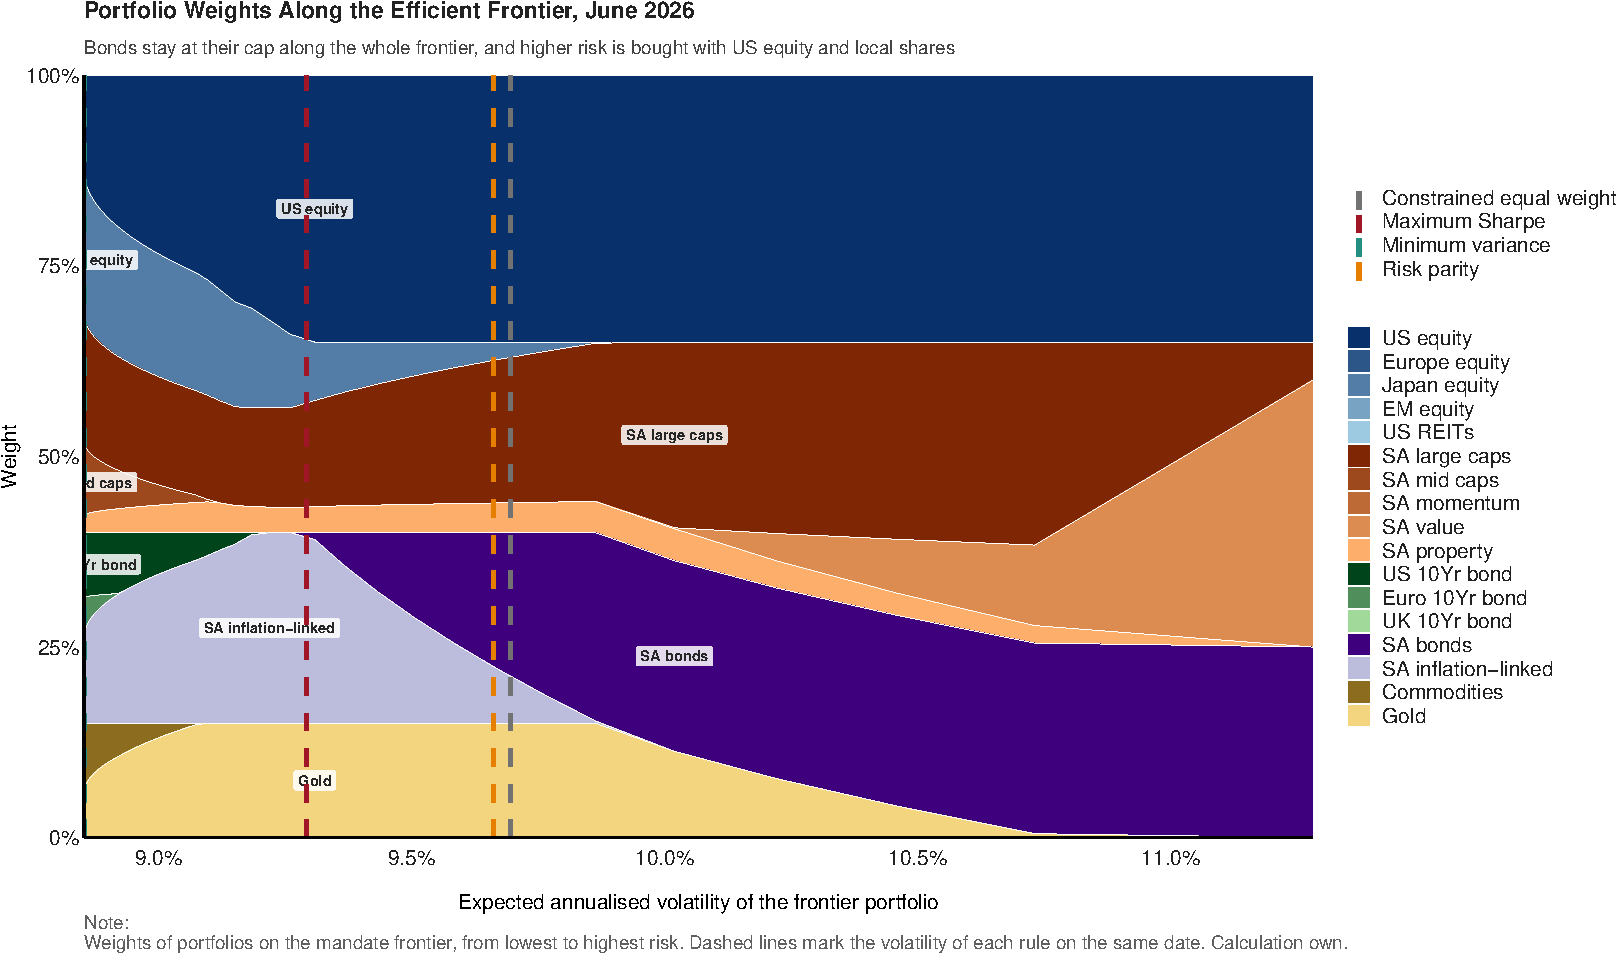
\includegraphics[width=1\linewidth]{Question4_files/figure-latex/q4_frontier_weights-1} 

}

\caption{Portfolio Weights Along the Efficient Frontier, June 2026}\label{fig:q4_frontier_weights}
\end{figure}

Bonds sit at their 25 percent cap along the entire frontier, so even the
least volatile mandate portfolio would hold more if it could. Moving up
the frontier, US equity rises from 13 percent to its 35 percent cap,
gold reaches its 15 percent class cap in the middle of the frontier and
then gives way to local shares, and the number of holdings falls from 10
at the lowest risk to 4 at the highest. Concentration therefore rises
with risk, which is the usual behaviour of mean-variance portfolios.
Minimum variance and maximum Sharpe sit on the frontier at its lower
end, while risk parity and the equal weight baseline sit slightly to the
right of maximum Sharpe, since they are not frontier portfolios.

\subsection{Random Portfolios Within the
Mandate}\label{random-portfolios-within-the-mandate}

Random portfolios give a benchmark that requires no optimisation at all.
A total of 20 000 portfolios are drawn by giving each asset class a
random budget within its limit and spreading it across the class at
random, and only the draws that also meet the single asset, global and
equity limits are kept.

\begin{figure}[H]

{\centering 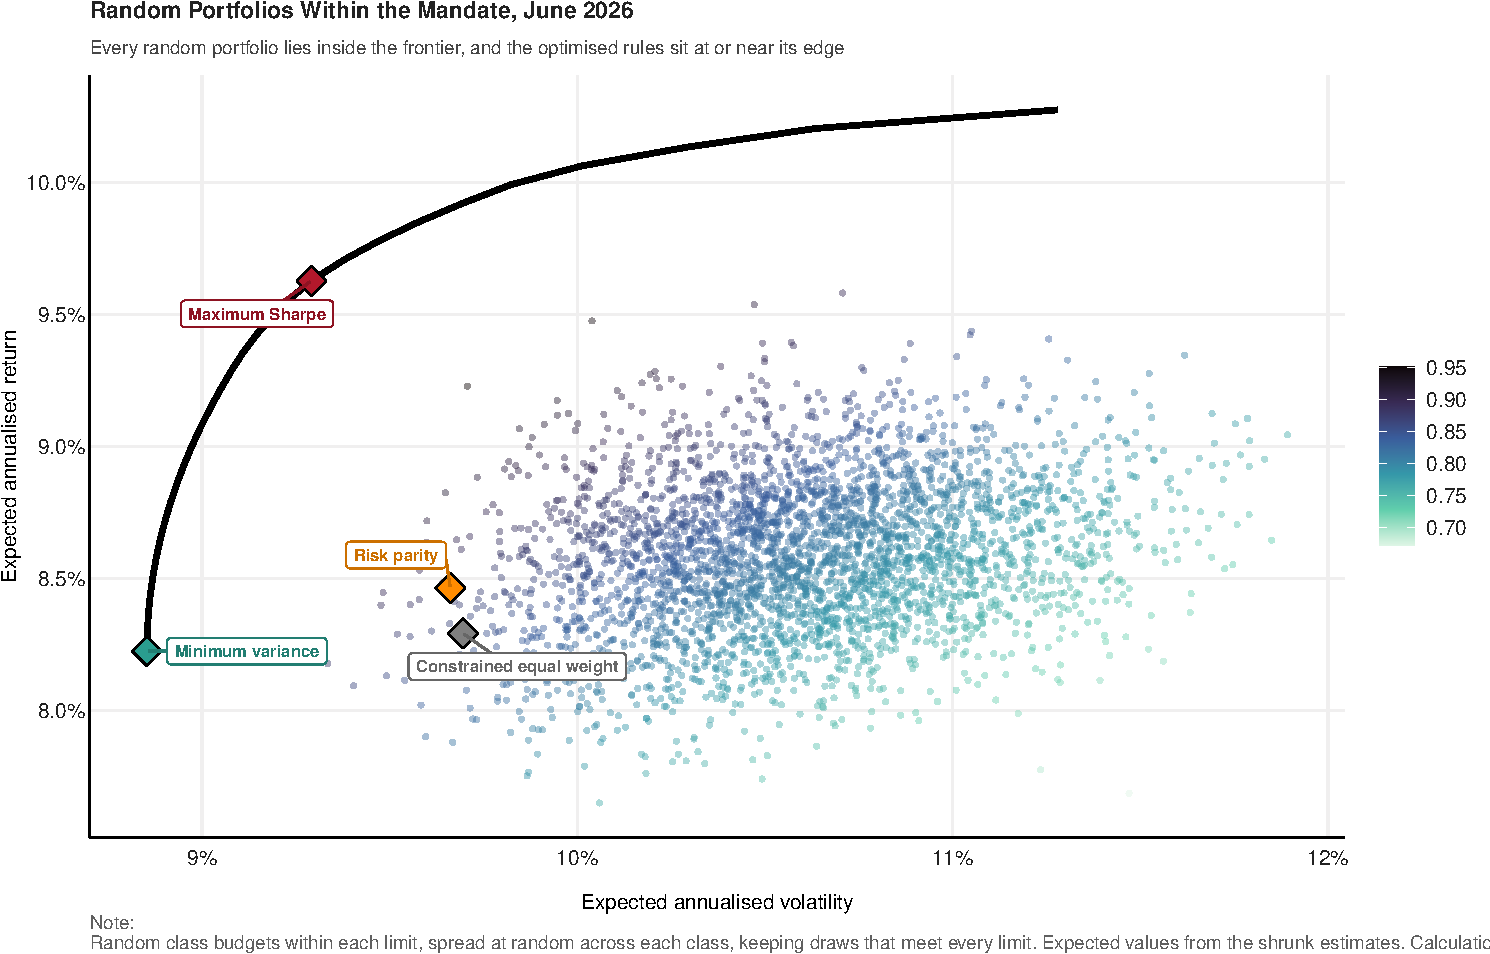
\includegraphics[width=1\linewidth]{Question4_files/figure-latex/q4_random-1} 

}

\caption{Random Portfolios Within the Mandate, June 2026}\label{fig:q4_random}
\end{figure}

Only 17.4 percent of the draws met every condition of the mandate, which
shows how much the limits restrict the choice. The 3 482 feasible
portfolios have expected volatility between 9.3 percent and 11.9
percent, and none reaches the frontier. The best of them earns 0.95
units of expected return per unit of risk, against 1.04 for the maximum
Sharpe portfolio, and the least volatile random portfolio is still
riskier than minimum variance. Risk parity and the equal weight baseline
sit at the low risk edge of the cloud, which is where a spread-out
portfolio with every class near its limit should fall.

\subsection{Capital Versus Risk}\label{capital-versus-risk}

A portfolio's weights describe where the money sits, while its risk
contributions describe where its ups and downs come from, and the two
can be very different. The paired bars below show, for each rule, the
share of capital in each family of assets next to that family's share of
portfolio risk, averaged over every rebalance date.

\begin{figure}[H]

{\centering 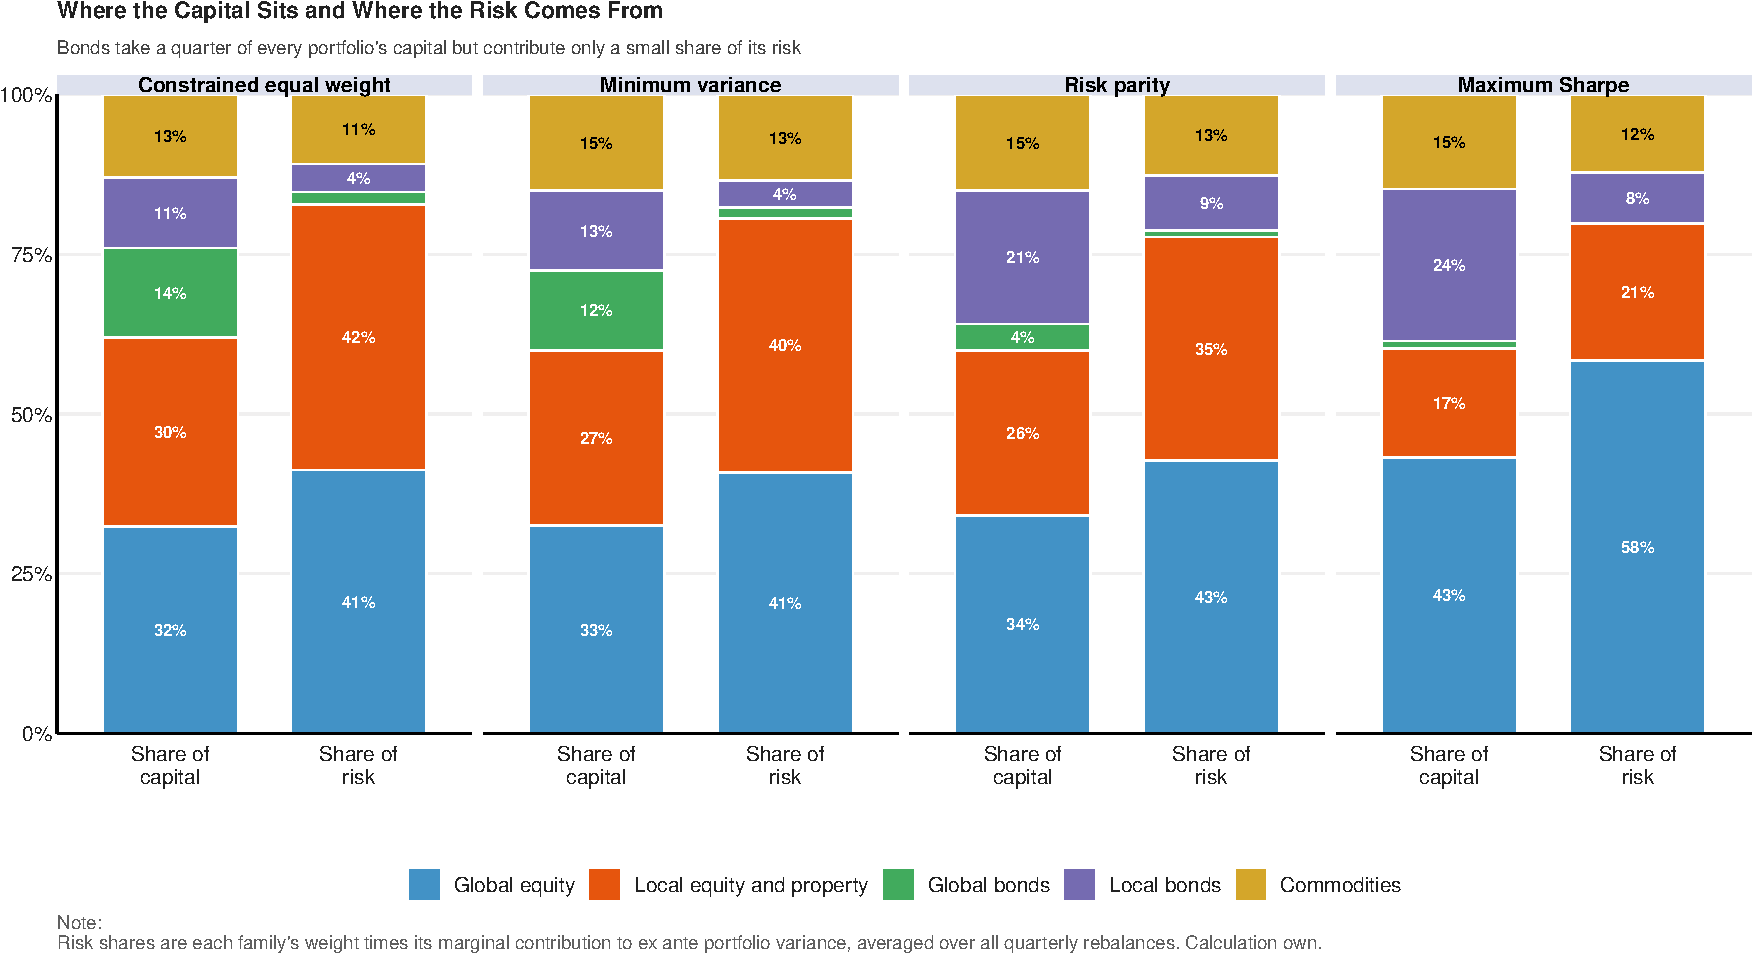
\includegraphics[width=1\linewidth]{Question4_files/figure-latex/q4_capital_risk-1} 

}

\caption{Where the Capital Sits and Where the Risk Comes From}\label{fig:q4_capital_risk}
\end{figure}

The bars show the central problem of a balanced fund. On average in the
risk parity portfolio, bonds hold 25 percent of the capital but
contribute only 10 percent of the risk, while equities hold 60 percent
of the capital and contribute 78 percent of the risk. The 25 percent
bond limit is what stops risk parity from balancing risk fully, since
equal risk would require far more in bonds. Maximum Sharpe is the
extreme case, with US equity alone contributing 48 percent of its risk
on average.

\subsection{The Latest Portfolios}\label{the-latest-portfolios}

The treemaps show the weights on the latest rebalance date, with each
tile's area in proportion to its weight and thick borders around each
family of assets.

\begin{figure}[H]

{\centering 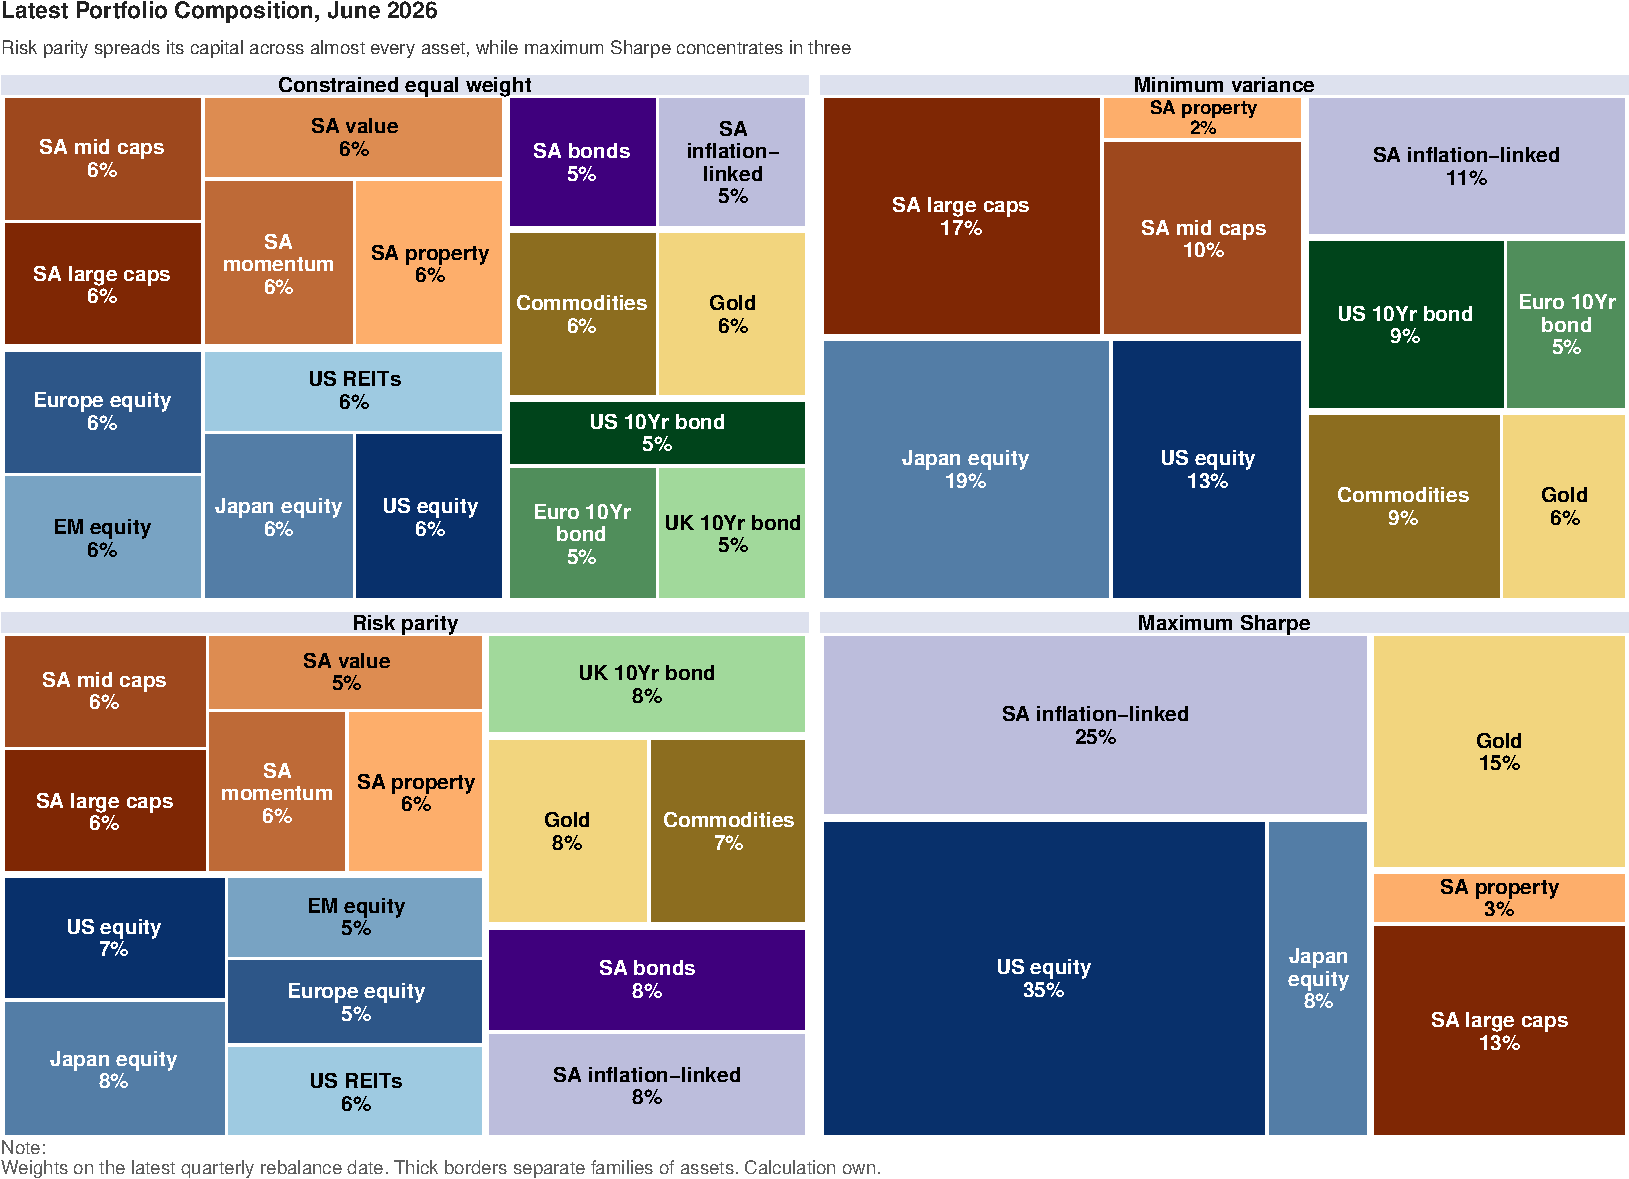
\includegraphics[width=1\linewidth]{Question4_files/figure-latex/q4_treemap-1} 

}

\caption{Latest Portfolio Composition, June 2026}\label{fig:q4_treemap}
\end{figure}

Risk parity holds 15 assets with no weight above 8 percent, and minimum
variance holds 10, led by Japan equity at 19 percent. Maximum Sharpe
holds only 6, with US equity at the 35 percent cap and the inflation
linked bonds and gold at their class caps, which is the usual tendency
of mean-variance optimisation to bet heavily on the assets with the
highest estimated returns.

The constrained equal weight baseline holds every eligible asset at
between 5.0 percent and 6.2 percent, since the 25 percent bond limit
forces it to hold less in each bond than in each equity index or
commodity. It is the simplest portfolio that respects the mandate and a
useful reminder of how far the optimisers move from it.

\subsection{How Hard the Mandate
Binds}\label{how-hard-the-mandate-binds}

The circular barplot shows how much of each limit every rule uses on
average across the rebalance dates, with the dashed ring marking a limit
that is fully used.

\begin{figure}[H]

{\centering 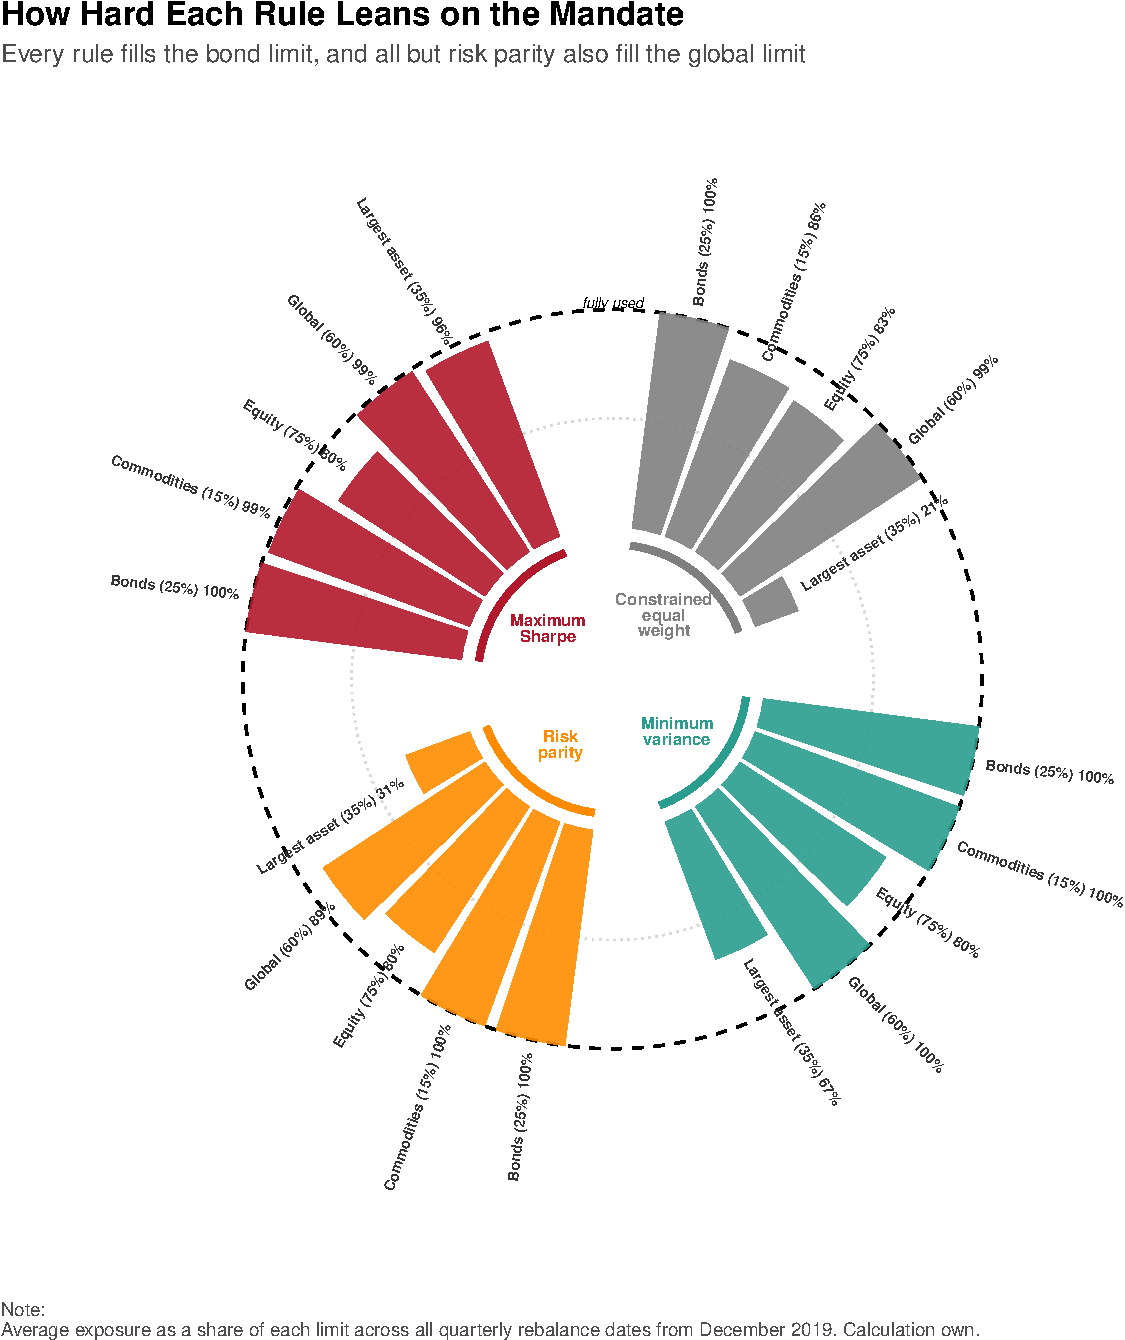
\includegraphics[width=1\linewidth]{Question4_files/figure-latex/q4_radial-1} 

}

\caption{How Hard Each Rule Leans on the Mandate}\label{fig:q4_radial}
\end{figure}

The bond limit is the most binding condition, used in full by every
rule, since bonds are the only low volatility asset class and every rule
wants as much of them as it can hold. The global limit binds for three
of the four rules, as offshore assets diversify the rand assets, and
risk parity uses 89 percent of it. The equity limit never binds.
Equities take whatever capital the other classes leave, and since the
rules fill the bond limit and most of the commodity limit, equities
settle near 60 percent, well below their 75 percent cap. The single
asset cap matters only for maximum Sharpe, which uses 96 percent of it
on average.

\section{\texorpdfstring{Backtest Performance
\label{Backtest}}{Backtest Performance }}\label{backtest-performance}

\subsection{Growth and Drawdowns}\label{growth-and-drawdowns}

The backtest holds each rule's weights for the quarter after each
rebalance, letting them drift with returns, and measures performance
from January 2020 to September 2026, a period that contains the Covid
crash, the 2022 rate shock and the strong markets of 2023 to 2026.

\begin{figure}[H]

{\centering 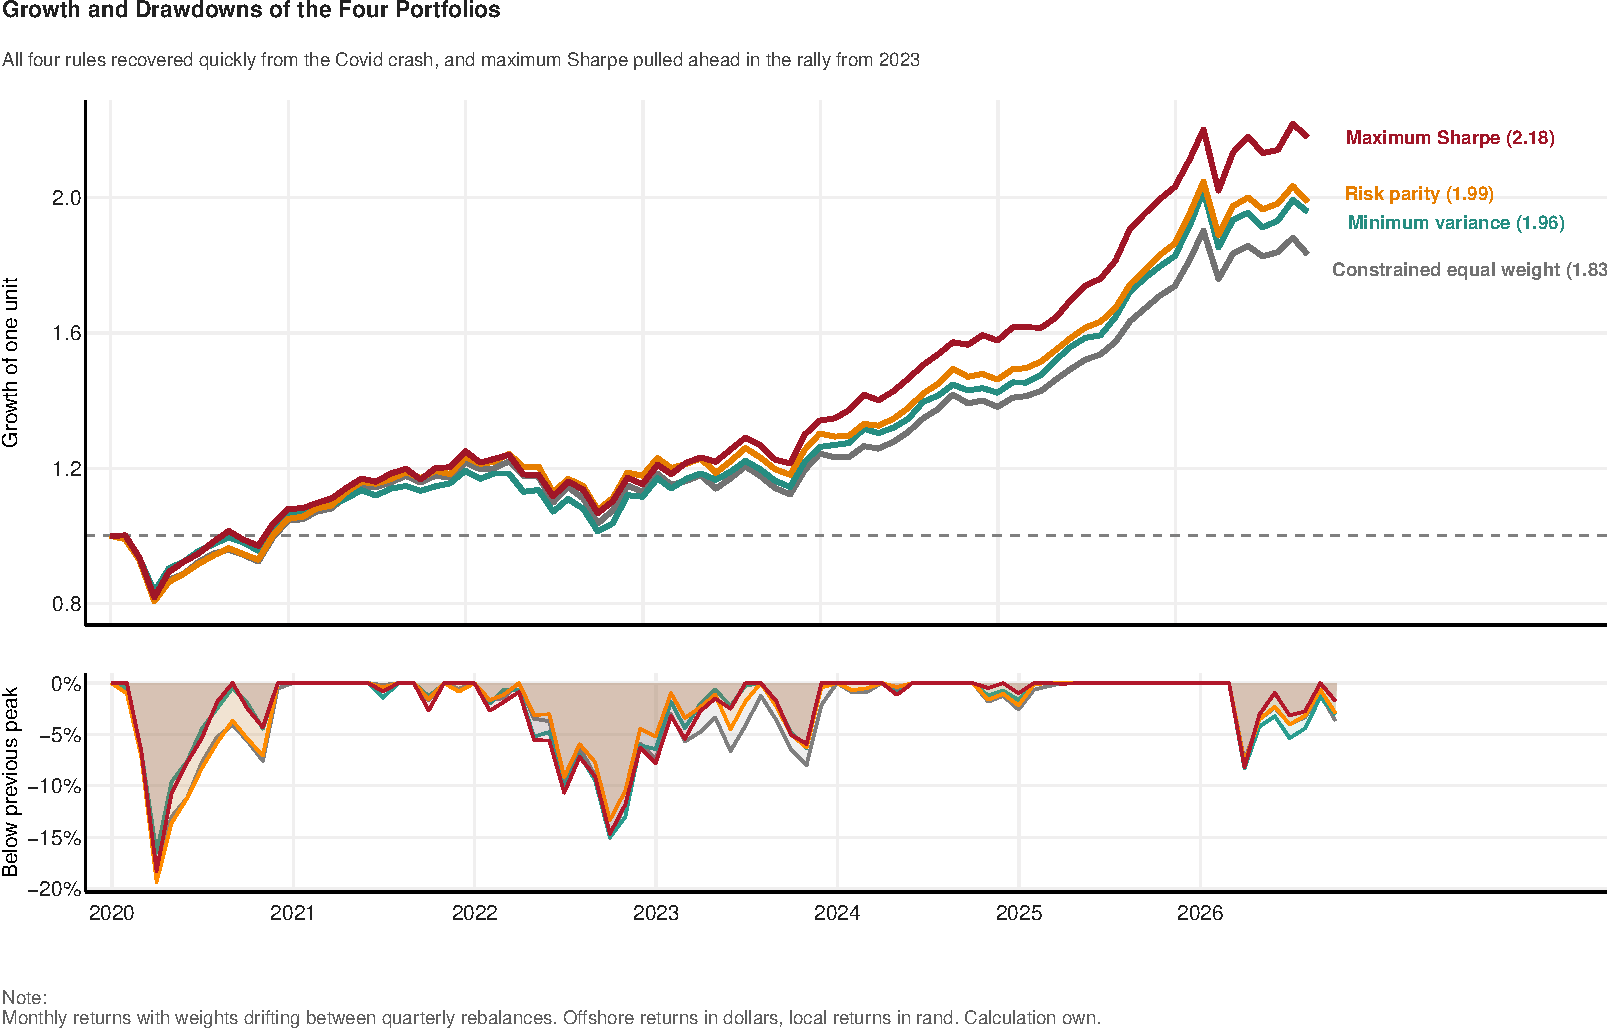
\includegraphics[width=1\linewidth]{Question4_files/figure-latex/q4_backtest-1} 

}

\caption{Growth and Drawdowns of the Four Portfolios}\label{fig:q4_backtest}
\end{figure}

Maximum Sharpe returned 12.2 percent a year, ahead of risk parity at
10.7 percent, minimum variance at 10.5 percent and the equal weight
baseline at 9.4 percent, with volatility between 11.4 percent and 12.0
percent for all four. The underwater chart shows that the Covid crash
produced the deepest losses for every rule, with risk parity's maximum
drawdown of 18.5 percent slightly deeper than minimum variance's 16.2
percent. The split by sub-period matters for a balanced fund. In the
stressed years from 2020 to 2022, risk parity returned the most, at 5.6
percent a year against 4.9 percent for maximum Sharpe, while maximum
Sharpe's lead comes entirely from the rally since 2023, when its 35
percent position in United States equity paid off.

\subsection{Monthly Return
Distributions}\label{monthly-return-distributions}

The rainclouds show the full distribution of monthly returns, with a
half density, a boxplot and every individual month as a dot.

\begin{figure}[H]

{\centering 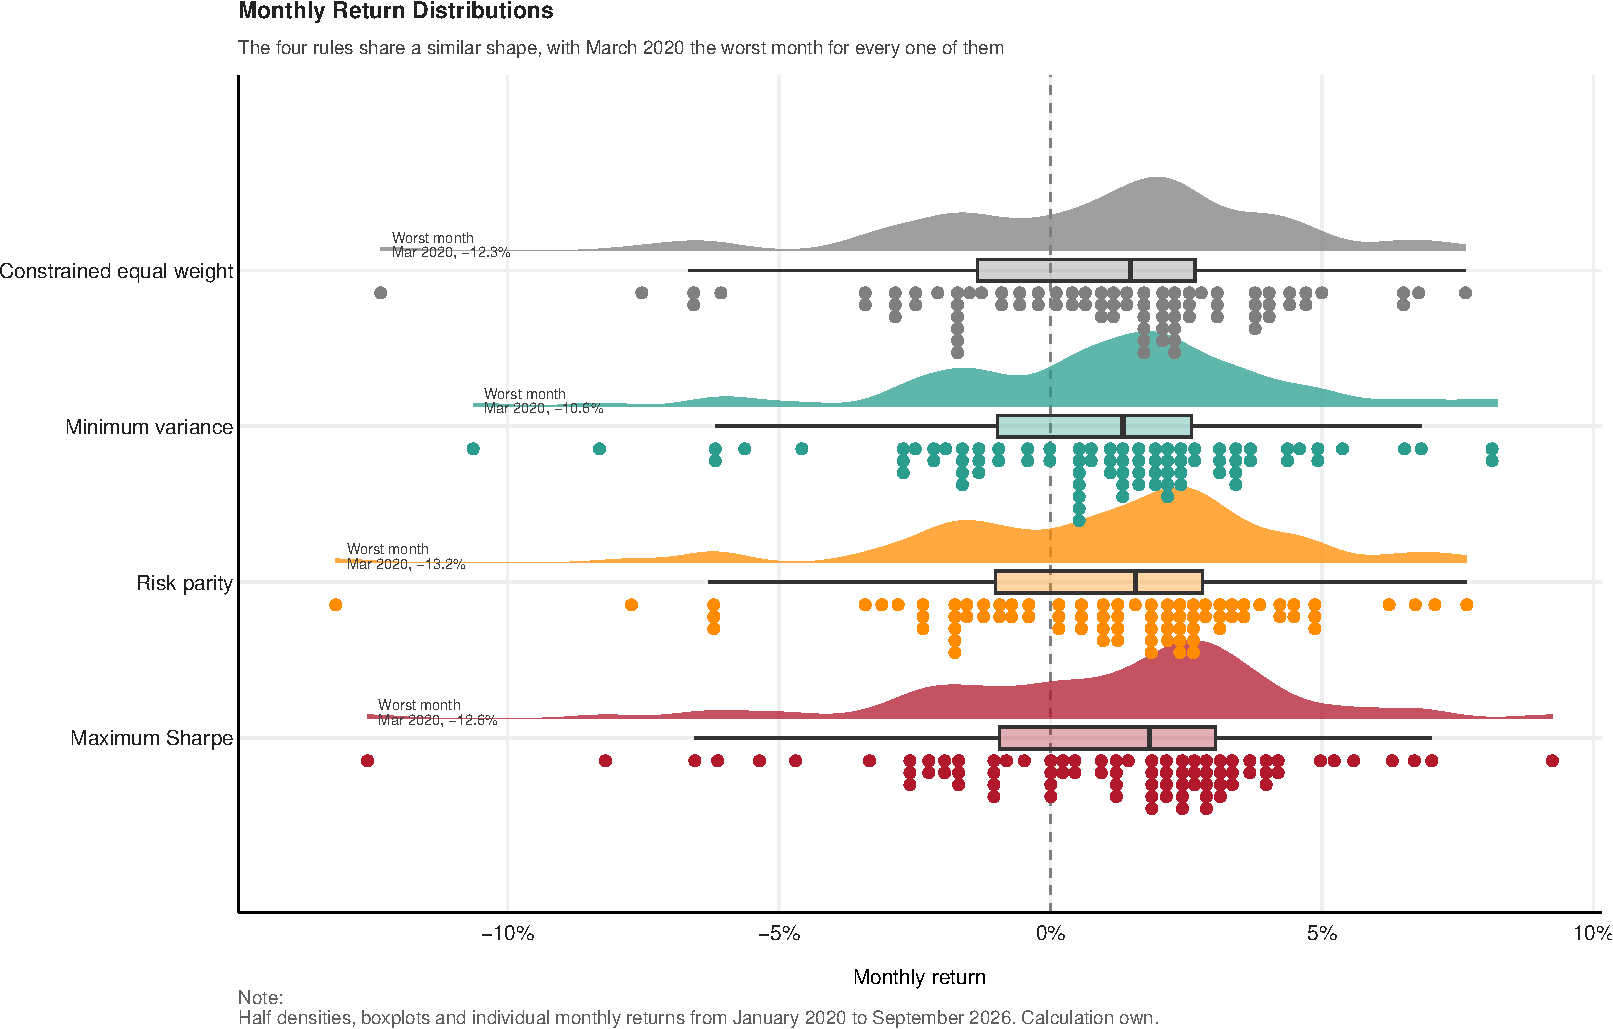
\includegraphics[width=1\linewidth]{Question4_files/figure-latex/q4_raincloud-1} 

}

\caption{Monthly Return Distributions}\label{fig:q4_raincloud}
\end{figure}

The distributions are close, which is expected when all four rules face
the same tight limits. The average of the worst five percent of months
ranges only from 7.4 percent to 7.9 percent, and the main difference
lies in the right tail, where maximum Sharpe has more strong months.

The tails differ more than the centres. The best month ranges from 7.6
percent to 9.2 percent across the rules, and the worst month, March 2020
for every rule, from -10.6 percent to -13.2 percent. The shared worst
month shows that the constraints leave every rule exposed to the same
equity crash, whatever its weighting scheme.

\subsection{Calendar Year Rankings}\label{calendar-year-rankings}

The bump chart ranks the rules by calendar year return, which shows how
consistently each one leads.

\begin{figure}[H]

{\centering 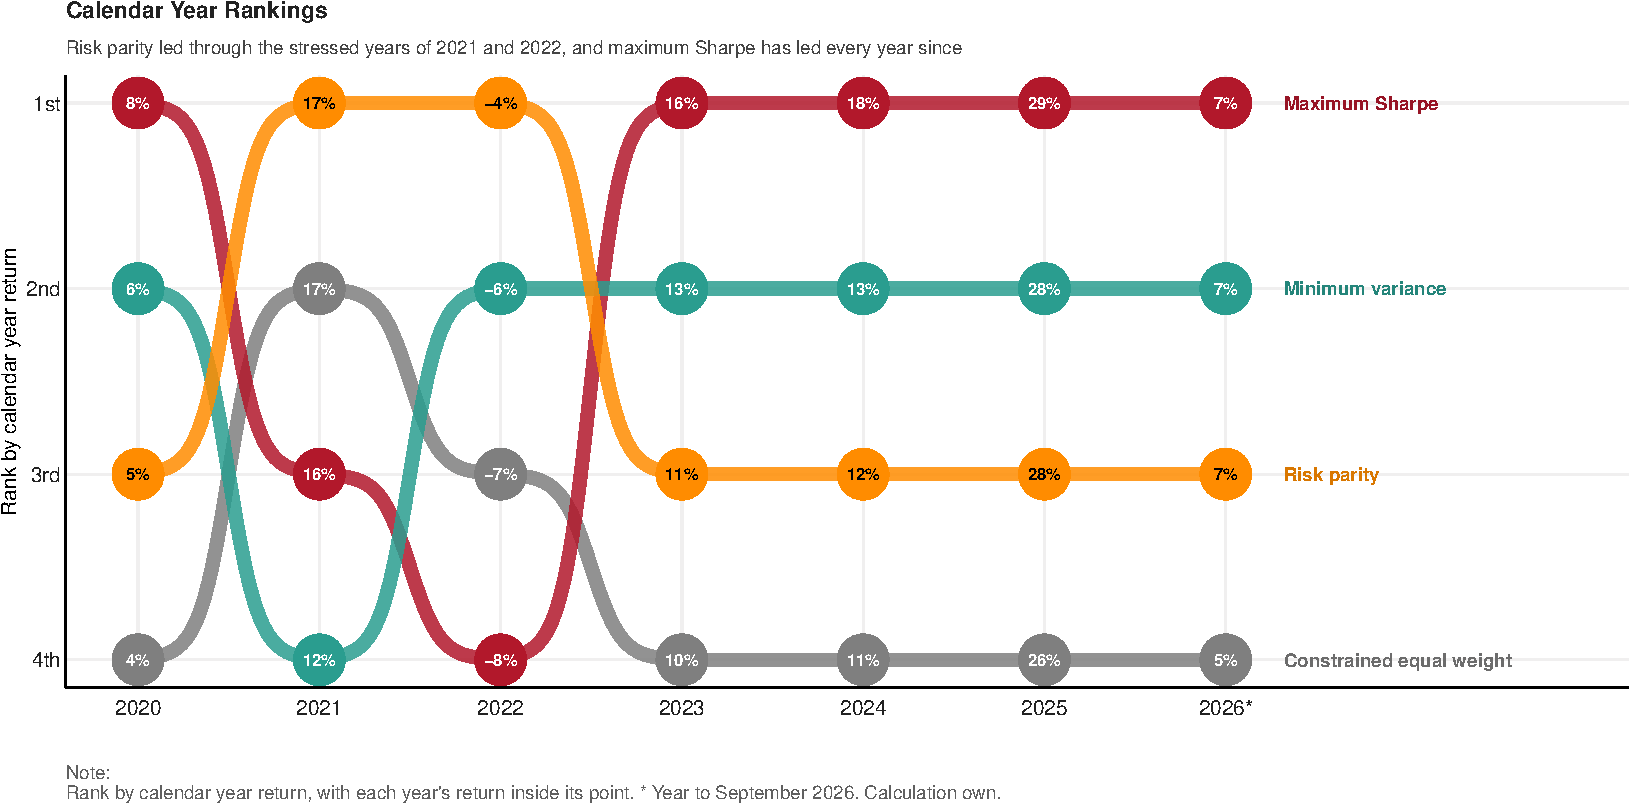
\includegraphics[width=1\linewidth]{Question4_files/figure-latex/q4_bump-1} 

}

\caption{Calendar Year Rankings}\label{fig:q4_bump}
\end{figure}

The ranks shift between regimes. Risk parity ranked first in 2021 and
2022, including the 2022 sell-off in which bonds and equities fell
together and its spread of risk helped most, while maximum Sharpe ranked
last in 2022 and first in every year since. No rule leads in every
environment, which is the case for choosing on robustness and not on the
latest ranking.

The differences between the rules are small in most years. In 2022, the
year bonds and equities fell together, the best and worst rules were
separated by 3.3 percentage points, and in 2025 by 2.9 points, so even
in the years with the largest gaps the choice of rule changes the
outcome by about three percentage points.

\section{\texorpdfstring{Scorecard and Recommendation
\label{Recommend}}{Scorecard and Recommendation }}\label{scorecard-and-recommendation}

\subsection{Scorecard}\label{scorecard}

The radar chart brings the measures together, scaling each so that the
outer ring is the best of the four rules.

\begin{figure}[H]

{\centering 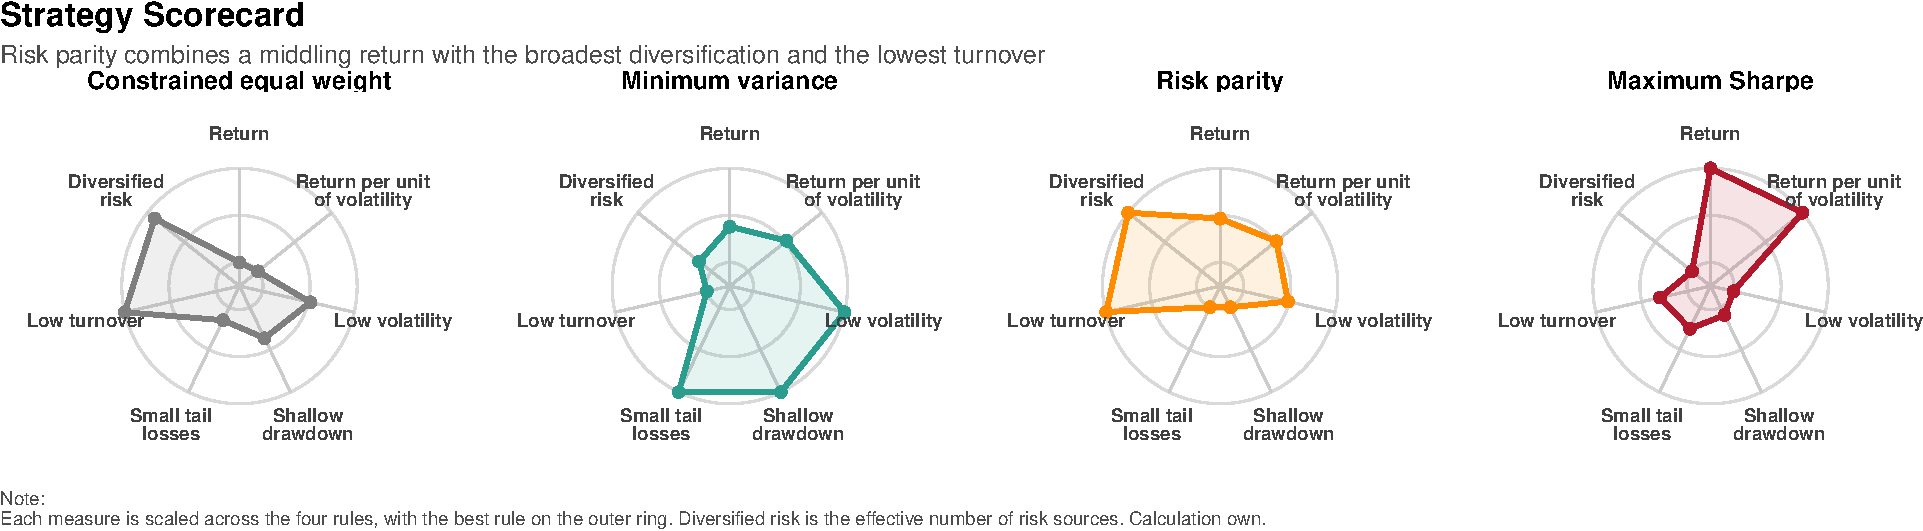
\includegraphics[width=1\linewidth]{Question4_files/figure-latex/q4_radar-1} 

}

\caption{Strategy Scorecard}\label{fig:q4_radar}
\end{figure}

The radar shows the trade-offs between the rules. Maximum Sharpe reaches
the outer ring on return and on return per unit of volatility but sits
near the centre on diversification and turnover. Minimum variance leads
on low volatility, shallow drawdowns and small tail losses. Risk parity
and the equal weight baseline are strongest on diversified risk and low
turnover, and risk parity also reaches the middle ring on return, which
gives it the most balanced shape of the four.

\subsection{Recommendation and
Robustness}\label{recommendation-and-robustness}

The recommended design is the constrained risk parity portfolio. It
delivered 10.7 percent a year, more than minimum variance and the equal
weight baseline at similar volatility, and it was the best rule in the
stressed years. Its risk is spread across an effective 12.8 sources,
against 3.4 for maximum Sharpe, and it trades only 2.8 percent of the
portfolio a quarter, against 6.5 percent for minimum variance, which
matters for an index fund that must keep trading costs low. It also does
not depend on expected returns. Maximum Sharpe's higher return rests on
its estimates of which assets will do best, and when those estimates are
not shrunk, its return falls to 11.6 percent, its drawdown deepens to
21.1 percent and its turnover rises to 6.8 percent.

The ranking is robust to the estimation choices. With no correlation
shrinkage, risk parity returns 11.1 percent and minimum variance 10.5
percent, and with twice the shrinkage the figures are 10.4 percent and
10.6 percent, so the conclusions do not hinge on that choice. Minimum
variance remains a defensible alternative for a client who values the
shallowest drawdown above everything else.

\FloatBarrier

\section{\texorpdfstring{Conclusion
\label{Conclusion}}{Conclusion }}\label{conclusion}

A balanced fund that meets every condition of the mandate can be built
from the universe provided, and four different rules all satisfy it on
every quarterly rebalance from December 2019. The mandate shapes the
result more than the choice of rule. The 25 percent bond limit binds for
every rule and stops any of them from balancing risk fully, the 60
percent global limit binds for most, and the equity limit never binds,
since filling the bond and commodity limits leaves equities near 60
percent. Within those limits, constrained risk parity offers the most
balanced combination of return, diversification and low turnover,
without relying on expected returns, and it held up best in the stressed
years of 2020 to 2022. Its main weakness is that bonds still contribute
only a small share of its risk, so the fund remains an equity-driven
portfolio, and offshore returns are measured in dollars, which means a
live fund would also carry rand exposure that this backtest does not
capture.

\bibliography{Tex/ref}





\end{document}
